\documentclass[10pt]{beamer}

\usetheme{CambridgeUS}
\usepackage[italian]{babel}
\usepackage[applemac]{inputenc}
\usepackage[T1]{fontenc}

\setbeamercovered{transparent}

\title{\textbf{ShirtShop}}
\subtitle{Negozio vendita on-line Magliette Personalizzate}
\author{Sistemi Informativi e Servizi in Rete}

\date{A.A. 2011-2012}

\begin{document}

\begin{frame}
	\maketitle
	Iora Marco 65574\\ Lorenzi Roberta 72361 \\ Piccinelli Andrea 83392\\
\end{frame}

\begin{frame}
	\frametitle{Obiettivi dell'applicazione}
	L'applicazione si propone di:
	\begin{itemize}
		\item <1-> essere una vetrina per la vendita di prodotti (magliette con stampe fronte e/o retro)
		on-line personalizzabili secondo qualunque esigenza
		\item <2-> fornire ai visitatori un'applicazione facile da usare per creare i propri prodotti
		personalizzati anche con stampe inviate dagli stessi clienti 
	\end{itemize}
\end{frame}

\begin{frame}
	\frametitle{Schema gerarchico degli utenti}
	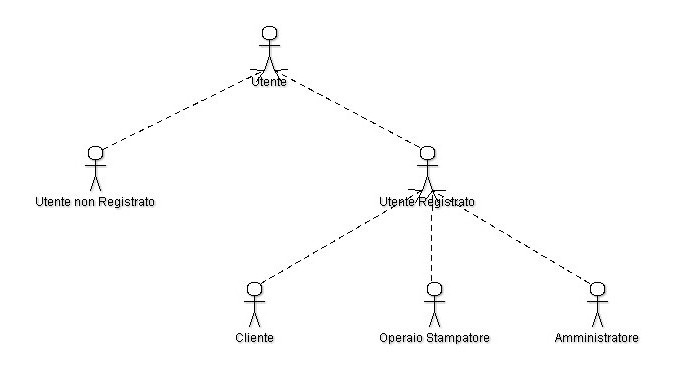
\includegraphics[height= 7cm]{Immagine/GerarchiaUtenti.jpg}
\end{frame}

\begin{frame}
	\frametitle{Diagramma dei casi d'uso: CLIENTE}
	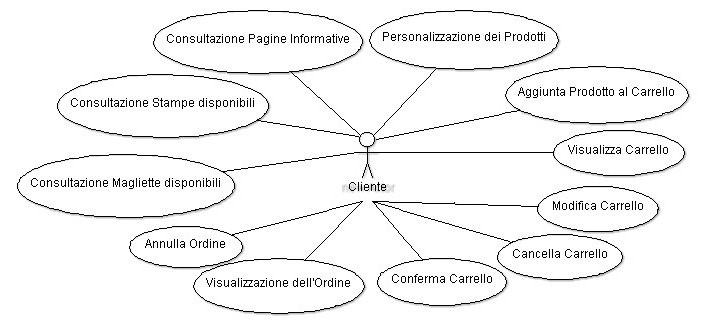
\includegraphics[height=5.5cm]{Immagine/CasoCliente.jpg}
\end{frame}

\begin{frame}
	\frametitle{Diagramma dei casi d'uso: OPERAIO STAMPATORE}
	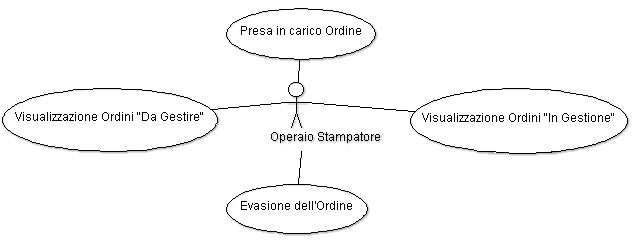
\includegraphics[height=4.5cm]{Immagine/CasoOperaioStampatore.jpg}
\end{frame}

\begin{frame}
	\frametitle{Diagramma dei casi d'uso: AMMINISTRATORE}
	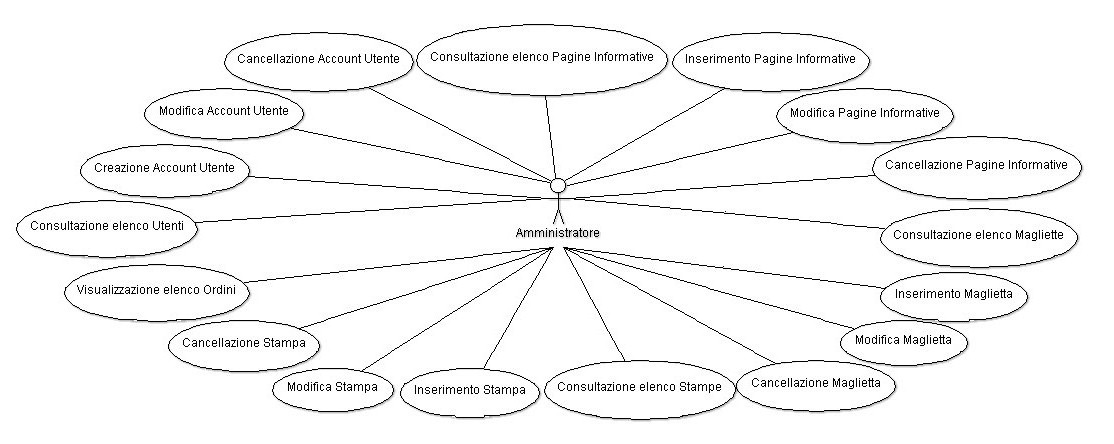
\includegraphics[height=5cm]{Immagine/CasoAmministratore.jpg}
\end{frame}

\begin{frame}
	\frametitle{Oggetti core e sotto-schemi core}
	\begin{center}
		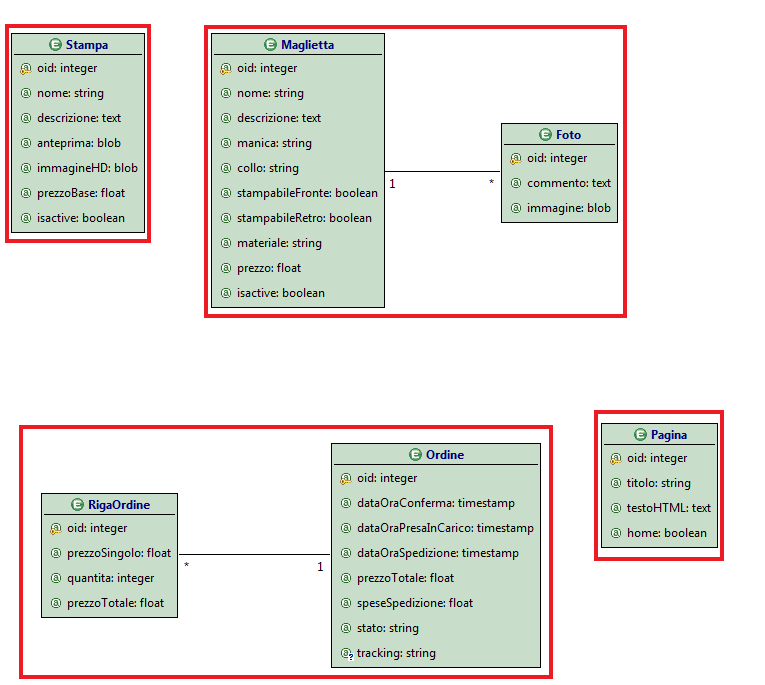
\includegraphics[height=7.5cm]{Immagine/Core.png}
	\end{center}
\end{frame}

\begin{frame}
	\frametitle{Sotto-schema di interconnesione}
	\begin{center}
		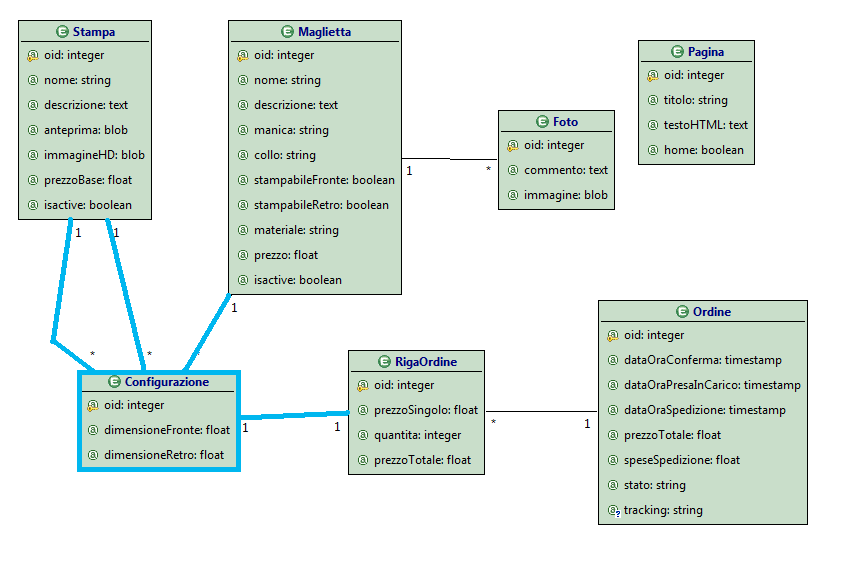
\includegraphics[height=7.5cm]{Immagine/Interconnessione.png}
	\end{center}
\end{frame}

\begin{frame}
	\frametitle{Sotto-schemi di accesso}
	\begin{center}
		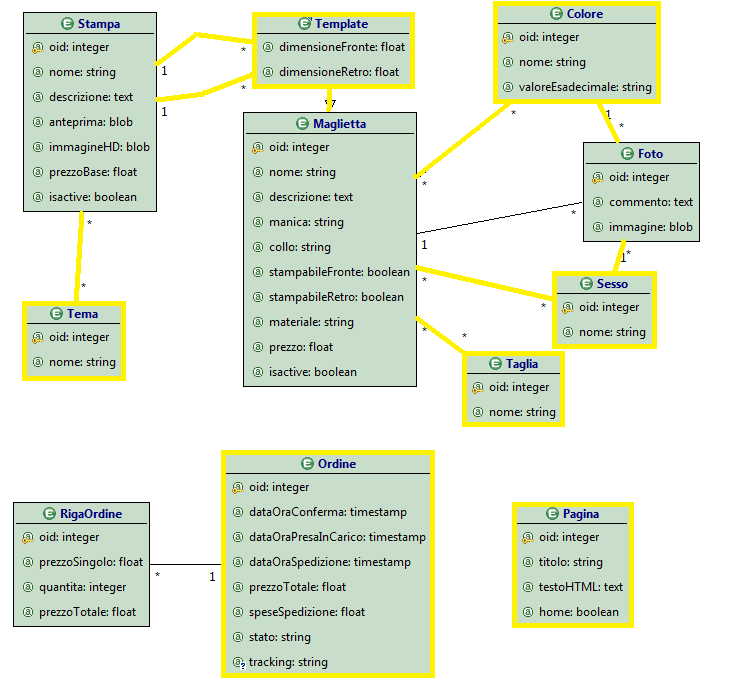
\includegraphics[height=7.5cm]{Immagine/Accesso.png}
	\end{center}
\end{frame}

\begin{frame}
	\frametitle{Sotto-schema di personalizzazione}
	\begin{center}
		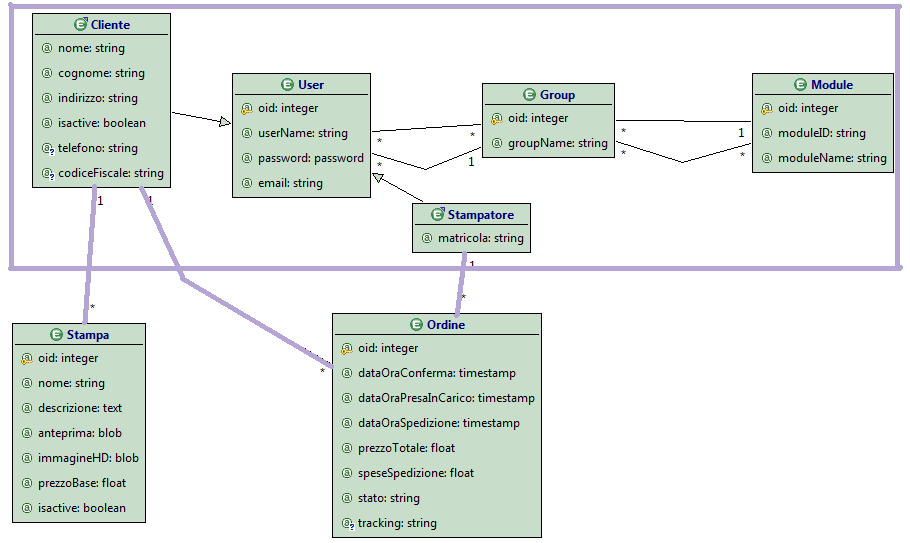
\includegraphics[height=6.5cm]{Immagine/Personalizzazione.png}
	\end{center}
\end{frame}

\begin{frame}
	\frametitle{Schema completo dei dati}
	\begin{center}
		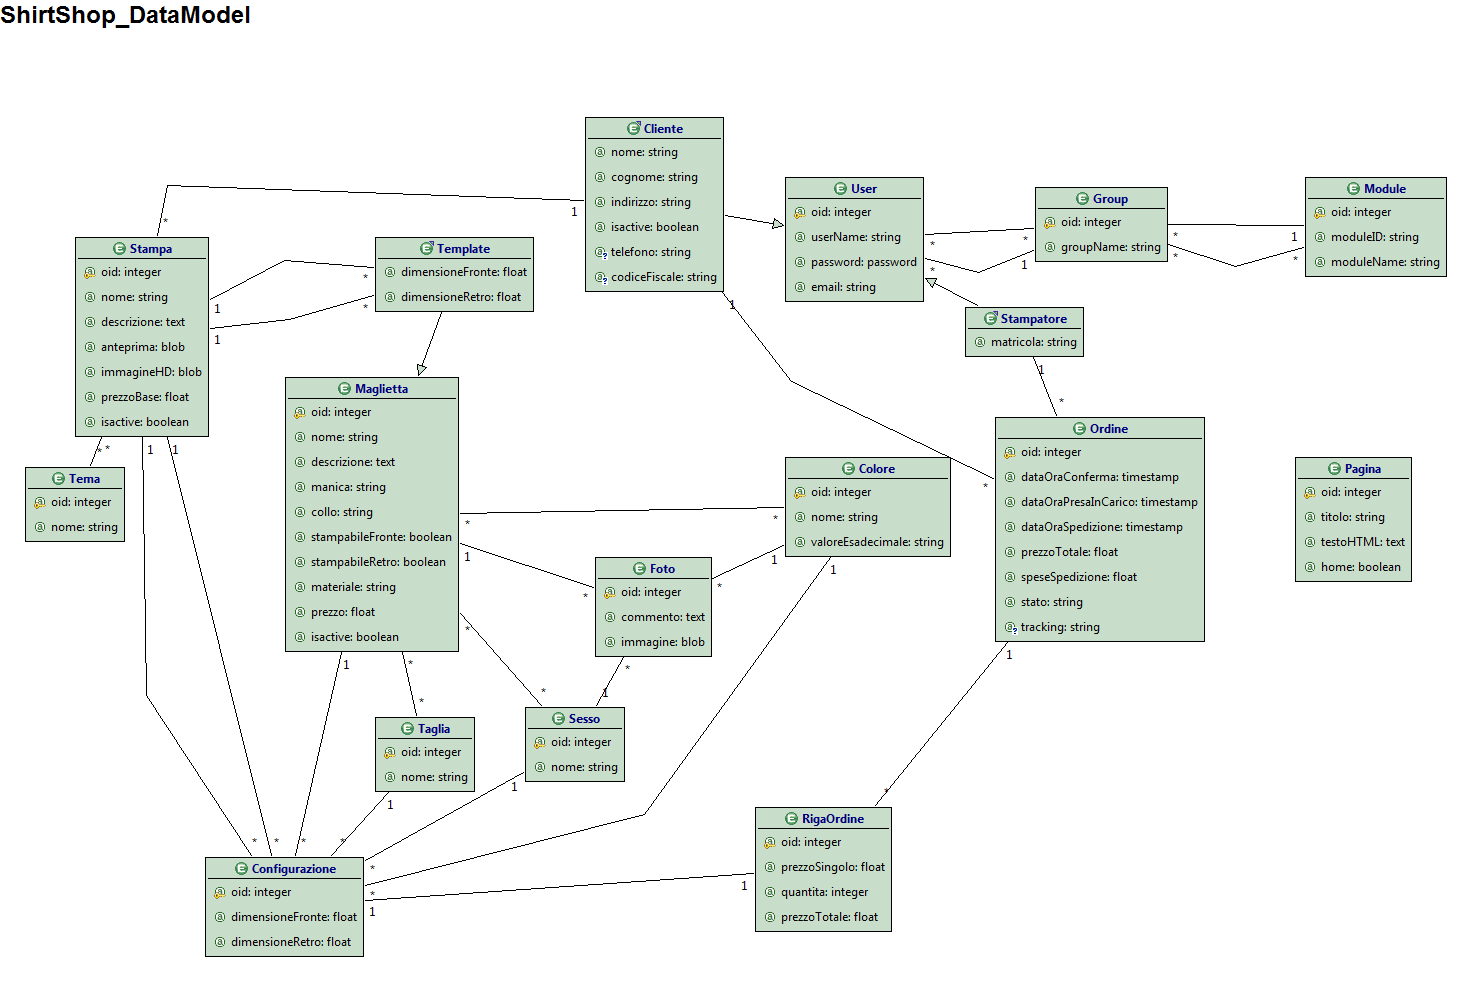
\includegraphics[height=7.5cm]{Immagine/SchemaCompletoDati.png}
	\end{center}
\end{frame}

\end{document}